\newdiscussion{Regular Expressions (Apr 13)}

A \emph{regular expression}, also known as ``regex,'' is a powerful feature of most modern programming languages.  Regexes allow programmers to build sophisticated string-manipulating functions with relative ease.  They are built on a simple, elegant formalism called \emph{finite automata}.  You may encounter some ugly regular expressions in the real world, but if you keep in mind that they are simple machines, you will always be able to understand them.~\footnote{For example, here are some seriously ugly regular expressions for validating URLs: \url{https://mathiasbynens.be/demo/url-regex}.}:

\section{Regular Expression Primer}

A regular expression is a sequence of text characters.  For example, the regular expression \texttt{aa} \emph{accepts} the string \scalainline{"aa"} and \emph{rejects} all other strings.  One way to think of \texttt{aa} is as a function that takes a \scalainline{String} as input and that returns a \texttt{Boolean} as output: \scalainline{true} if the string is \scalainline{"aa"} and \scalainline{false} otherwise.

A regular expression is equivalent to a class of \emph{state machines} called a \emph{nondeterministic finite automaton}, or NFA.  NFAs can be drawn as a directed graph, and having this graph in your head helps understand what the regular expression algorithm does.  The rules are simple.  (1) Every possible change in the state of the machine (a ``transition'') is uniquely determined by the source state and input symbol.  (2) The machine ``accepts'' if and only if a sequence of input symbols results in the NFA ending in an ``accepting'' state (a circle with double lines).

Here's the NFA for the regular expression \texttt{aa}:

\begin{center}
  \begin{tikzpicture}[->,>=stealth',shorten >=1pt,auto,node distance=2.8cm,
                      semithick]
    \tikzstyle{every state}=[fill=none,draw=black,text=black]

    \node[initial,state] (1)              {$q_0$};
    \node[state]         (2) [right of=1] {$q_1$};
    \node[state,accepting]         (3) [right of=2] {$q_2$};
    \path (1) edge              node {a} (2)
          (2) edge              node {a} (3);
  \end{tikzpicture}
\end{center}

\subsection{Analogy: Hunt the Wumpus}

Think of this graph as a maze\footnote{See \url{https://en.wikipedia.org/wiki/Hunt_the_Wumpus}}.  You start at $q_0$, the circle at the beginning of the maze.  Your goal is to get to $q_2$, the circle at the end of the maze (the one with double lines).  You can follow paths (arrows) in the direction that they point, but not the other way.  And unfortunately, this maze is filled with evil, dangerous creatures!  Now, you're no fool.  You brought a map!  If your map is right, you make it out alive.  If not, you meet your doom in the maze.  Is your map any good?

Your map is the input string \scalainline{"aa"}.  Start at $q_0$.  The map says to go down path \scalainline{"a"}.  OK, that takes us to $q_1$.  After that, the map says to go down path \scalainline{"a"}.  Great!  This brings us to $q_2$.  We made it out!  The maze ``accepts'' the map.

What if we had the map \scalainline{"bb"}?  We'd start at $q_0$ and go to $q_1$.  But then the map says to take the path \scalainline{"b"}.  There is no \scalainline{"b"} path.  We're doomed! The maze ``rejects'' the map and the wumpus (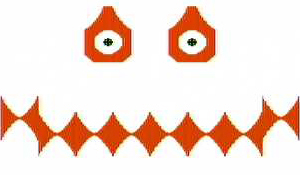
\includegraphics[width=0.5cm]{wumpus.jpg}) eats you.

\subsection{One Caveat (Among Many) to My Beautiful Analogy}

Note that my analogy assumes that our input string and our regular expression both start and end in the same place.  This fact would imply that a regular expression matches an \emph{entire input string}.  In practice, it is often useful to write regular expressions that match a \emph{substring}.  In many regular expression implementations, one denotes whole-string matches by prepending the regex with the \texttt{\^{}} character and appending it with the \texttt{\$} character.  For example, \texttt{aa} becomes \texttt{\^{}aa\$}.

Scala's \scalainline{regex.pattern.matcher(str).matches()} (where \scalainline{regex} is a regex and \scalainline{str} is an input string) always matches the entire string, so \texttt{\^{}} and \texttt{\$} are unnecessary.  Other Scala regex methods do not work this way.  You should be careful that the function you use has the semantics that you want, so please check the Scala docs if you are unsure.

\section{Discussion Programming Tasks}

We are going to do programming tasks 2 and 5 in class.  They are:

\begin{itemize}

  \item Define the regular expression \scalainline{time}, which only matches times written as five-character strings \texttt{HH:MM}, where the hours range from 00--23 and the minutes from 00--59.
 
  \item Define the regular expression \scalainline{comment}, which only matches strings that start with \texttt{/*} and end with \texttt{*/}.

\end{itemize}

\section{Homework Hint for the Parity-Checking Regular Expression}

The last regex is a tricky one.  It helps if you know a certain arithmetical law~\footnote{Which is somewhere on this page: \url{https://en.wikipedia.org/wiki/Parity_(mathematics)}}.
